\section{Method}

As illustrated in Figure~\ref{fig:overview}, our approach treats alpha mining as an agentic research workflow rather than a one-shot factor construction procedure. 
Given market context and user-provided seeds, a multi-agent system produces a complete mining trajectory that records hypothesis generation, controllable factor construction, code implementation, and backtesting-based evaluation. 
We first describe the end-to-end mining workflow that instantiates and evaluates a single trajectory (Section~\ref{sec:4.1}). 
Building on these evaluated trajectories, we then introduce an evolutionary optimization scheme that iteratively improves mining quality via a self-evolution process (Section~\ref{sec:4.2}).
\begin{figure}[htbp]
    \centering
    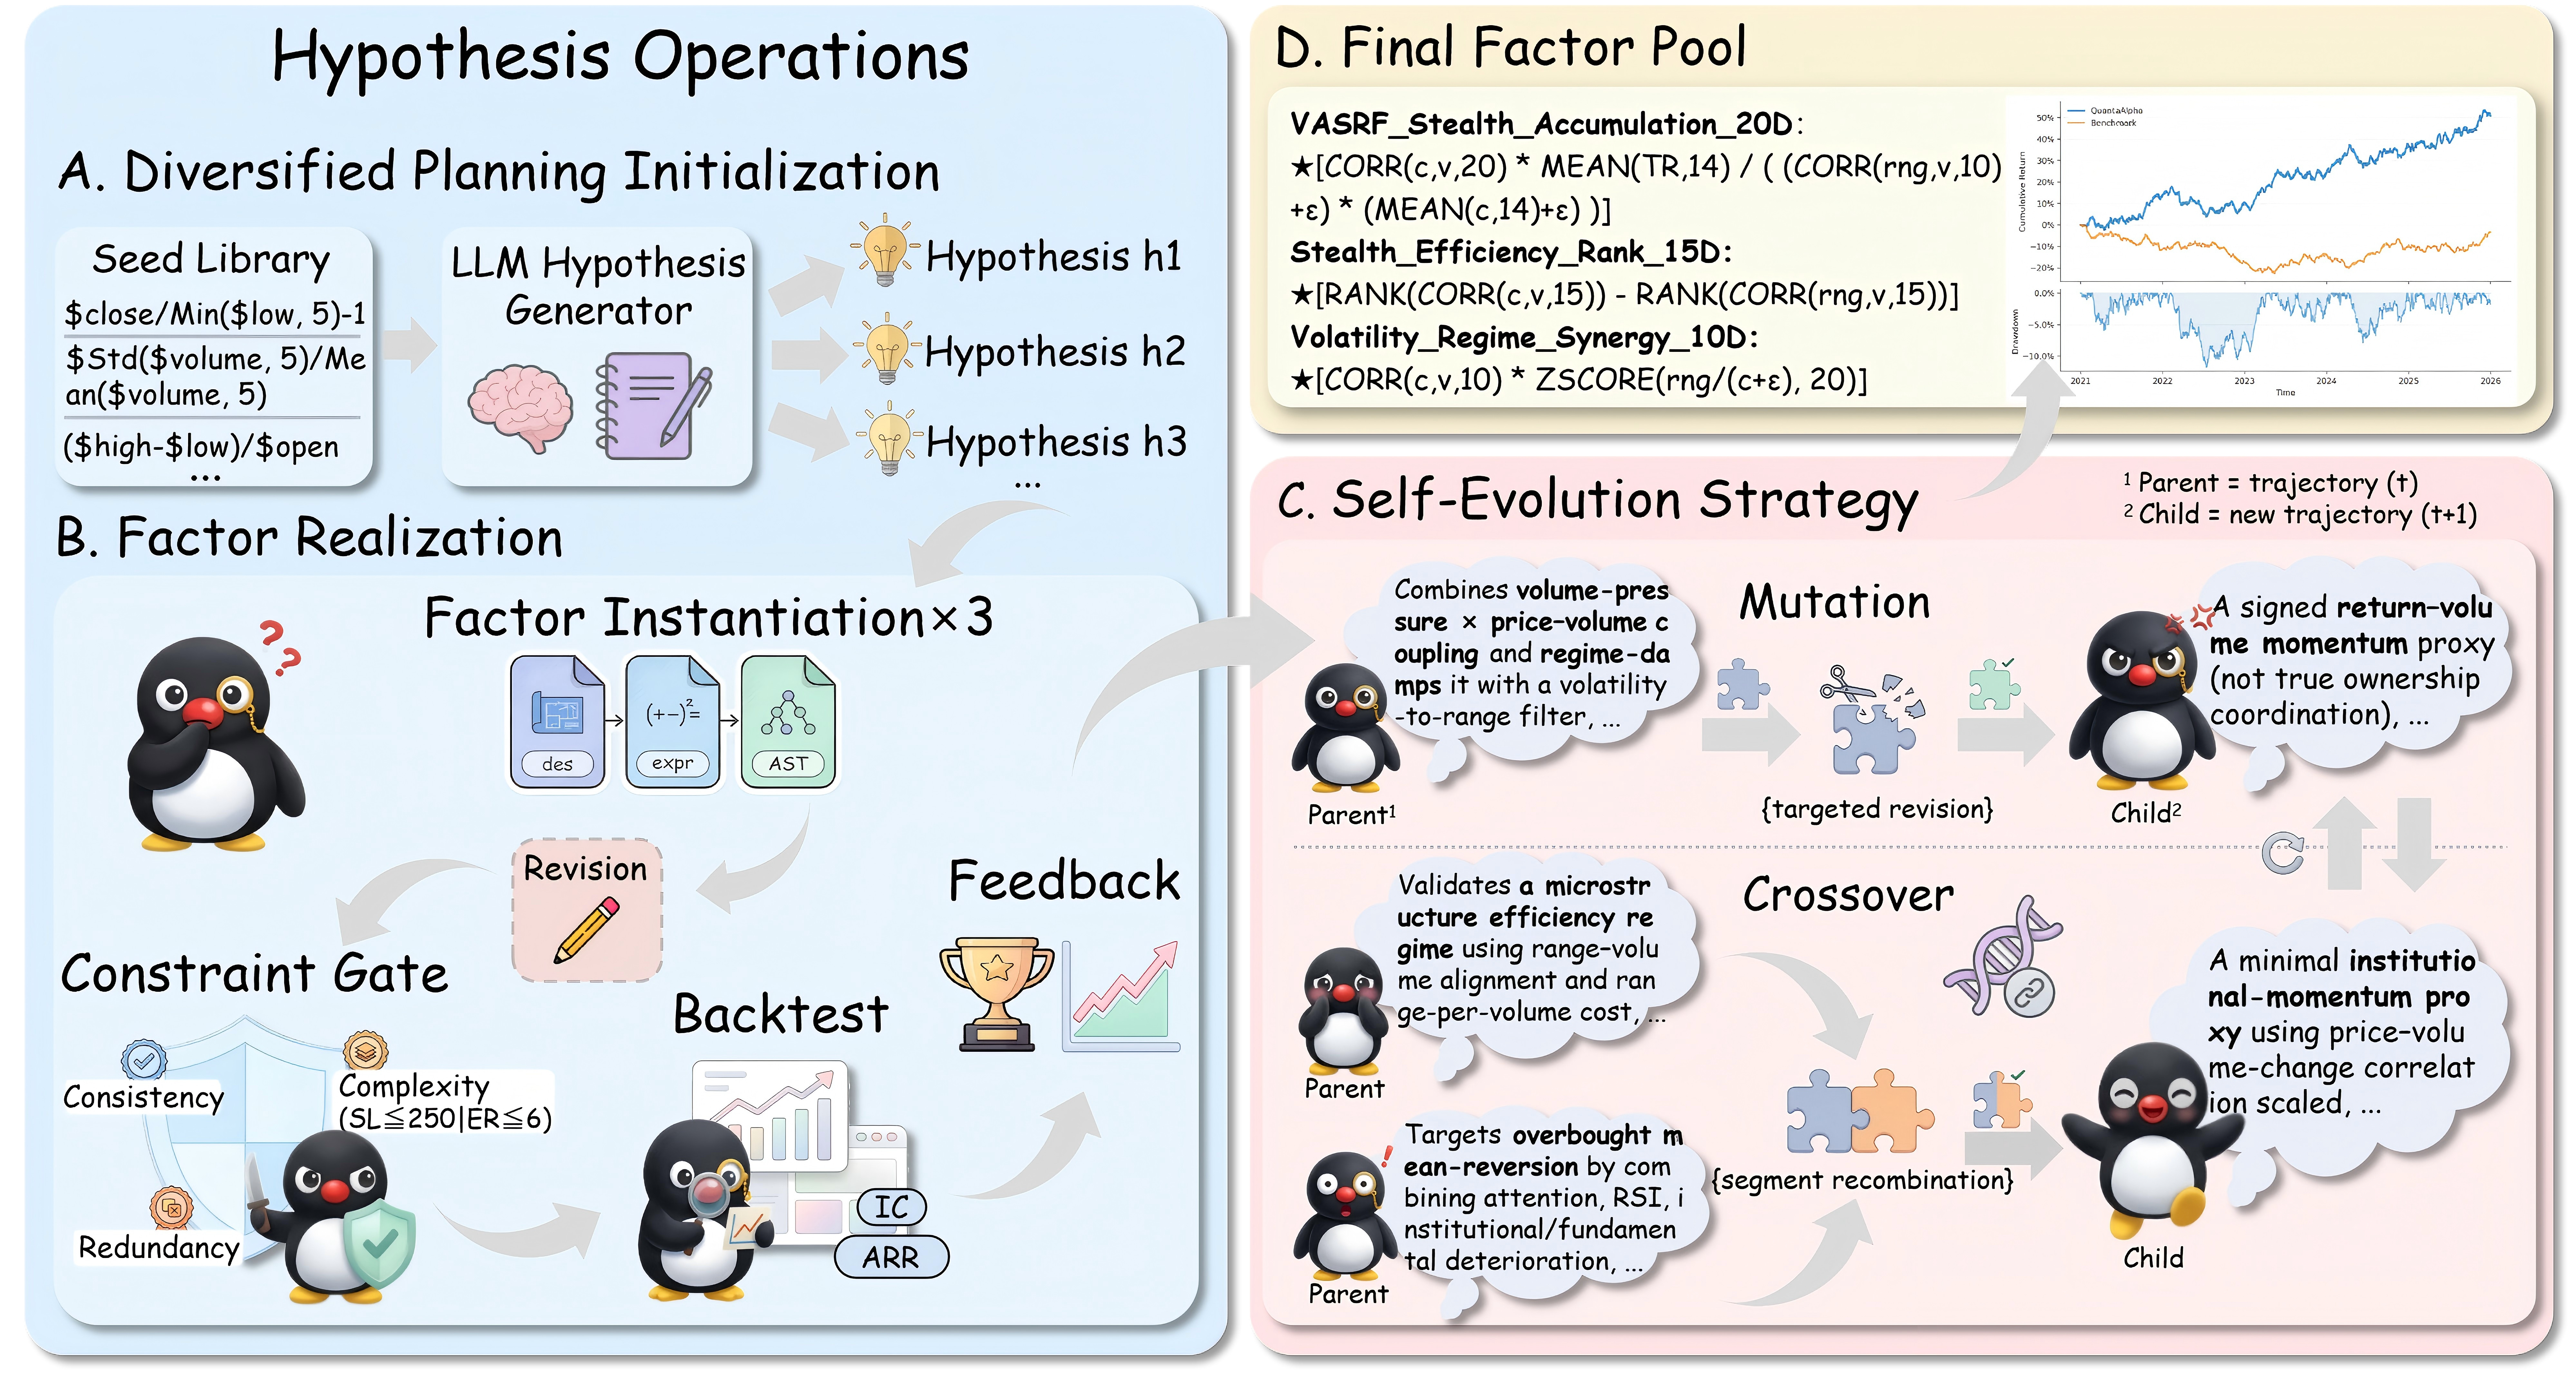
\includegraphics[width=1\textwidth]{images/overview.jpg}
    \caption{\textbf{Overview of the QuantaAlpha framework}. Our approach consists of four core components: (A) Diversified Planning Initialization to generate candidate hypotheses, (B) Factor Realization that iteratively instantiates hypotheses into executable factors with constraint gating, (C) Self-Evolution that applies mutation and crossover over evaluated trajectories, and (D) A Final Factor Pool that consolidates validated effective factors.}
    \label{fig:overview}
\end{figure}
\subsection{Alpha Mining Process} 
\label{sec:4.1}
A standalone alpha mining process involves a sequential progression starting from hypothesis generation, followed by factor creation and concluding with backtesting-based evaluation. We translate this process into the collaborative efforts of multiple agents, each responsible for a specific task at different stages of the workflow. 

\subsubsection{Hypothesis Generation}
We use the idea agent $\mathcal{A}{i}$ to generate market hypotheses via structured knowledge integration. Conditioned on (i) observations from current market conditions or previous mining trajectories, (ii) domain priors from financial theories and empirical evidence, and (iii) parametric specifications (e.g., ``10-day high/low''), $\mathcal{A}{i}$ produces actionable hypotheses that describe candidate market mechanisms and serve as the input to subsequent factor generation.

\subsubsection{Controllable Factor Construction}
To effectively instantiate hypothesis-driven factors, we need a robust mechanism to align implementations with domain hypotheses. However, directly generating factor code is brittle, often suffering from syntax errors, dependency mismatches, and semantic drift, causing a mismatch between the code and the hypothesis.To address these limitations, We introduce an intermediate symbolic representation based on a standardized operator library $\mathcal{O}$ and an Abstract Syntax Tree (AST). This abstraction bridges high-level market intent and low-level implementation, enabling controllable construction, structural validation, and reliable compilation.
\paragraph{Factor Generation} Given a hypothesis $h \in \mathcal{H}$ and raw features $\mathcal{X}$, the factor agent $\mathcal{A}_{f}$ generates a symbolic expression $f \in \mathcal{F}$ over the operator library and parses it into an AST as the intermediate representation. Concretely, it first maps $h$ to a structured semantic description $d$ that formalizes the intended mechanism into discrete operators, while concurrently instantiating operational parameters—such as look-back windows and thresholds—from either prescribed parameters in $h$ or heuristic defaults anchored in domain expertise.
Conditioned on $d$, the agent then assembles an operator composition into a symbolic expression $f$ and parses it into an AST, denoted as $T(f)$. In $T(f)$, leaf nodes bind to raw feature fields (e.g., \texttt{\$high}, \texttt{\$volume}) and internal nodes correspond to operator instances from $\mathcal{O}$ (e.g., \texttt{TS\_MIN}($\cdot$), \texttt{SMA}($\cdot$), \texttt{RANK}$(\cdot)$), thereby rendering the computational dependencies and data flow fully transparent.
Finally, the agent translates the validated symbolic form into executable code $c$ via compilation; when compilation fails due to implementation issues, an LLM-based repair step is triggered to regenerate a consistent implementation while preserving the semantics of $f$. This design ensures that code generation remains anchored to an explicit symbolic specification rather than unconstrained free-form generation.
\paragraph{Consistency Verification} We enforce semantic consistency across representations to prevent drift during generation. Specifically, we apply an LLM-based verifier to assess (i) alignment among the hypothesis $h$, semantic description $d$, and symbolic expression $f$, and (ii) faithfulness between the symbolic definition $f$ and the generated code $c$. The verifier returns a consistency decision under fixed criteria. If it fails, we rewrite the inconsistent component(s) by regenerating $d$ and $f$ or repairing $c$ until the check passes or a maximum retry budget is reached.
\paragraph{Complexity and Redundancy Control} We further regularize factor generation with explicit structural constraints to promote parsimony and novelty. For complexity, we compute
\begin{equation}
\mathcal{C}(f)
= \alpha_1 \cdot SL(f)
+ \alpha_2 \cdot PC(f)
+ \alpha_3 \cdot \log\!\bigl(1 + |F_f|\bigr),
\label{eq:factor_complexity}
\end{equation}
where $SL(f)$ measures symbolic length, $PC(f)$ counts free parameters (e.g., window sizes), and $F_f$ is the set of raw features used by $f$. For redundancy, we quantify structural similarity via AST matching. Given two factors $f_i$ and $f_j$ with ASTs $T(f_i)$ and $T(f_j)$, we define $s(f_i,f_j)$ as the size of their largest common isomorphic subtree:
\begin{equation}
s(f_i,f_j)
=\max_{\substack{S_i \subseteq T(f_i), S_j \subseteq T(f_j), S_i \cong S_j}} |V(S_i)|.
\end{equation}
Here, $S_i$ and $S_j$ range over subtrees of $T(f_i)$ and $T(f_j)$, respectively, $S_i \cong S_j$ denotes subtree isomorphism, and $|V(S_i)|$ is the number of nodes in $S_i$. For a candidate factor $f$, we compute its maximum similarity against an existing alpha zoo $\mathcal{Z}$ as 
\begin{equation}
S(f)=\max_{\phi\in\mathcal{Z}} s(f,\phi).
\label{eq:max_similarity}
\end{equation}
We reject and rewrite any factor that violates the prescribed complexity or redundancy limits, promoting parsimonious generation while avoiding near-duplicate structures.
\subsubsection{Factor Evaluation} 
The evaluation agent $\mathcal{A}_{e}$ assesses factors via a standardized backtesting system. The protocol covers three complementary aspects: predictive capability metrics for forecasting effectiveness, return performance metrics for profit-generating potential under a fixed execution setting, and risk control metrics for stability and robustness across market conditions. Beyond factor scoring, the agent maintains an evaluation history that records outcomes and summarizes systematic patterns among successful and failed factors.

\subsection{Evolutionary Alpha Mining}
\label{sec:4.2}
We improve alpha discovery via iterative optimization over mining trajectories. Starting from user-provided seed factors, we generate a diversified set of initial hypotheses. We then run the end-to-end mining workflow in Section~\ref{sec:4.1} to turn each hypothesis into an evaluated mining trajectory, forming an initial trajectory pool $\mathcal{T}_0=\{\tau_1^0,\tau_2^0,\ldots,\tau_{N_{init}}^0\}$. We then apply an iterative evolution process to obtain progressively improved factors.
\subsubsection{Diversified Planning Initialization}
\label{sec:4.2.1}
Let $\mathcal{Z}_0$ denote the user-provided seed factors (or seed ideas). 
We employ an initialization agent $\mathcal{A}_0$ to propose a diversified set of initial hypotheses $\mathcal{H}^{0}=\{h^{0}_1,\ldots,h^{0}_{N_{init}}\}$. The agent is instructed to maximize complementarity among hypotheses at both semantic and structural levels, e.g., varying signal sources (price vs.\ volume), time scales (short-term vs.\ long-term), and mechanism types (momentum vs.\ mean-reversion or regime-conditioned triggers). For each $h^{0}_i \in \mathcal{H}^{0}$, we run the mining workflow in Section~\ref{sec:4.1} and obtain a mining trajectory $\tau^{0}_i$.
This diversified initialization expands the effective search frontier by providing broad starting coverage in the hypothesis space. As a result, the subsequent evolutionary process can explore multiple promising regions in parallel, significantly reducing the risk of premature convergence to a suboptimal local optimum.
\subsubsection{Self-Evolution}
\label{sec:4.2.2}
The goal of self-evolutionary updates is to guide the alpha mining system to search for better trajectories based on existing ones. Specifically, we apply trajectory-level operators to existing mining trajectories to generate improved trajectories as demonstrations. These demonstrations provide imitation learning priors that bias subsequent trajectory generation toward effective decisions. In practice, we instantiate the update with two evolutionary primitives, Mutation and Crossover, which revise a single trajectory or recombine complementary sub-trajectories, respectively. Each iteration $i$ yields a new trajectory generation $\mathcal{T}_i$, and factor quality improves progressively across iterations (see Figure~\ref{fig:case_study} in Appendix for a case study).
\paragraph{Mutation}
Given a mining trajectory $\tau \in \mathcal{T}_{i-1}$, the primitive first performs self-reflection to diagnose sub-optimal decision node that most significantly accounts for the low terminal reward,
denoted by an index $k\in\{0,\ldots,n-1\}$. 
We then rewrite only the localized action (or a short local segment) while keeping the remaining steps unchanged:
\begin{equation}
\tau_{child}=\big(s_0,a_0,\ldots,s_k,\mathrm{Refine}(a_k),s_{k+1}',a_{k+1}',\ldots,s_n'\big), 
\label{eq:controlled_mutation}
\end{equation}
where the prefix up to $s_k$ is frozen, and the remaining steps are regenerated by the agent conditioned on this fixed prefix to preserve trajectory coherence. Depending on the localized fault, the rewrite may update the hypothesis, the symbolic expression under the operator library, or the compiled code, and can introduce mechanism-level changes such as altering the time scale, or adding regime conditions.
\paragraph{Crossover}
Crossover aims to exploit and inherit validated components by recombining complementary sub-trajectories from high-quality parents. At iteration $i-1$, we select a parent subset $\mathcal{P}_{i-1}\subseteq \mathcal{T}_{i-1}$ based on trajectory reward (Eq.~\ref{eq:traj_reward}). Given $k$ parent trajectories $\tau^{(1)},\ldots,\tau^{(k)}\in\mathcal{P}_{i-1}$, Crossover synthesizes a new child trajectory by composing high-performing segments from different parents:
\begin{equation}
\tau_{\mathrm{child}} = \mathrm{Crossover}\big(\tau^{(1)},\ldots,\tau^{(k)}\big).
\label{eq:crossover}
\end{equation}
Operationally, the primitive identifies specific trajectory segments that consistently contribute to high cumulative rewards—such as hypothesis templates, factor construction patterns, or strategic repair actions—and merges them into a single, highly coherent sequence.
This recombination mimics the human practice of combining complementary strengths from different solutions, while providing a more credible lineage by explicitly inheriting decisions that have been validated in previously successful trajectories.

